The charged Higgs decays to \PQc quark and \PQs antiquark. Reconstruction and
identification of jets coming from these quarks is very important to reconstruct 
the mass of charged Higgs ($\mHp$). We reconstruct ($\mHp$) before and after 
kinematic fit as follows:
\begin{itemize}[leftmargin=*]
    \item {\bf{$\mHp$ reconstruction before kinematic fitting}}: The jets are 
        reconstructed and selected as described in Section~\ref{s:jet_reco}. Events are
        required to have at least 4 jets. We use \PQb tagging as described in Section~\ref{s:bTag}
        to tag two jets as \PQb-tagged jet. The jets are sorted in descending order of 
	\PQb-discriminator values and the first two jets are considered as \PQb jets. If an event 
	contains exactly 4 jets then the other 2 non \PQb jets are used to evaluate $\mjj$. However, 
	if an event contains more than 4 jets, then the non \PQb jets are sorted in descending order 
	of $\pt$ and two highest $\pt$ non \PQb jets are used to evaluate $\mjj$. The invariant 
        mass ($\mjj$) distribution after \PQb jet selection as described in Section~\ref{s:secEvtSel} 
	is shown in Figures~\ref{subfig:mjj_muBTag},~\ref{subfig:mjj_eleBTag} for data and
        background, and in Figures~\ref{subfig:mjj_sig_btag_mu},~\ref{subfig:mjj_sig_btag_ele} for 
	all charged Higgs signal samples for \mujets and \ejets channel respectively.
    
    \item {\bf{$\mHp$ reconstruction after kinematic fitting}}: The kinematic 
        fit is performed on the reconstructed jets of Section~\ref{s:jet_reco}, as
        described in Chapter~\ref{s:KinFit}, in the semi-leptonic decay mode of
        \ttbar where \PW boson from one of the \PQt quarks decays leptonically 
        and \PW boson from the other \PQt quark decays hadronically. 
	The $\mjj$ distribution from two light jets after kinematic fit selection is 
	shown in Figures~\ref{subfig:mjj_kfit_muKinFit} ,~\ref{subfig:mjj_kfit_eleKinFit} for data 
	and background, and in Figures~\ref{subfig:mjj_sig_kfit_mu},~\ref{subfig:mjj_sig_kfit_ele} for 
	all charged Higgs signal samples for \mujets and \ejets channel respectively. 
    \end{itemize}
\begin{figure}
    \centering  
    \subfigure[With reconstructed jets \label{subfig:mjj_sig_btag_mu}]
    {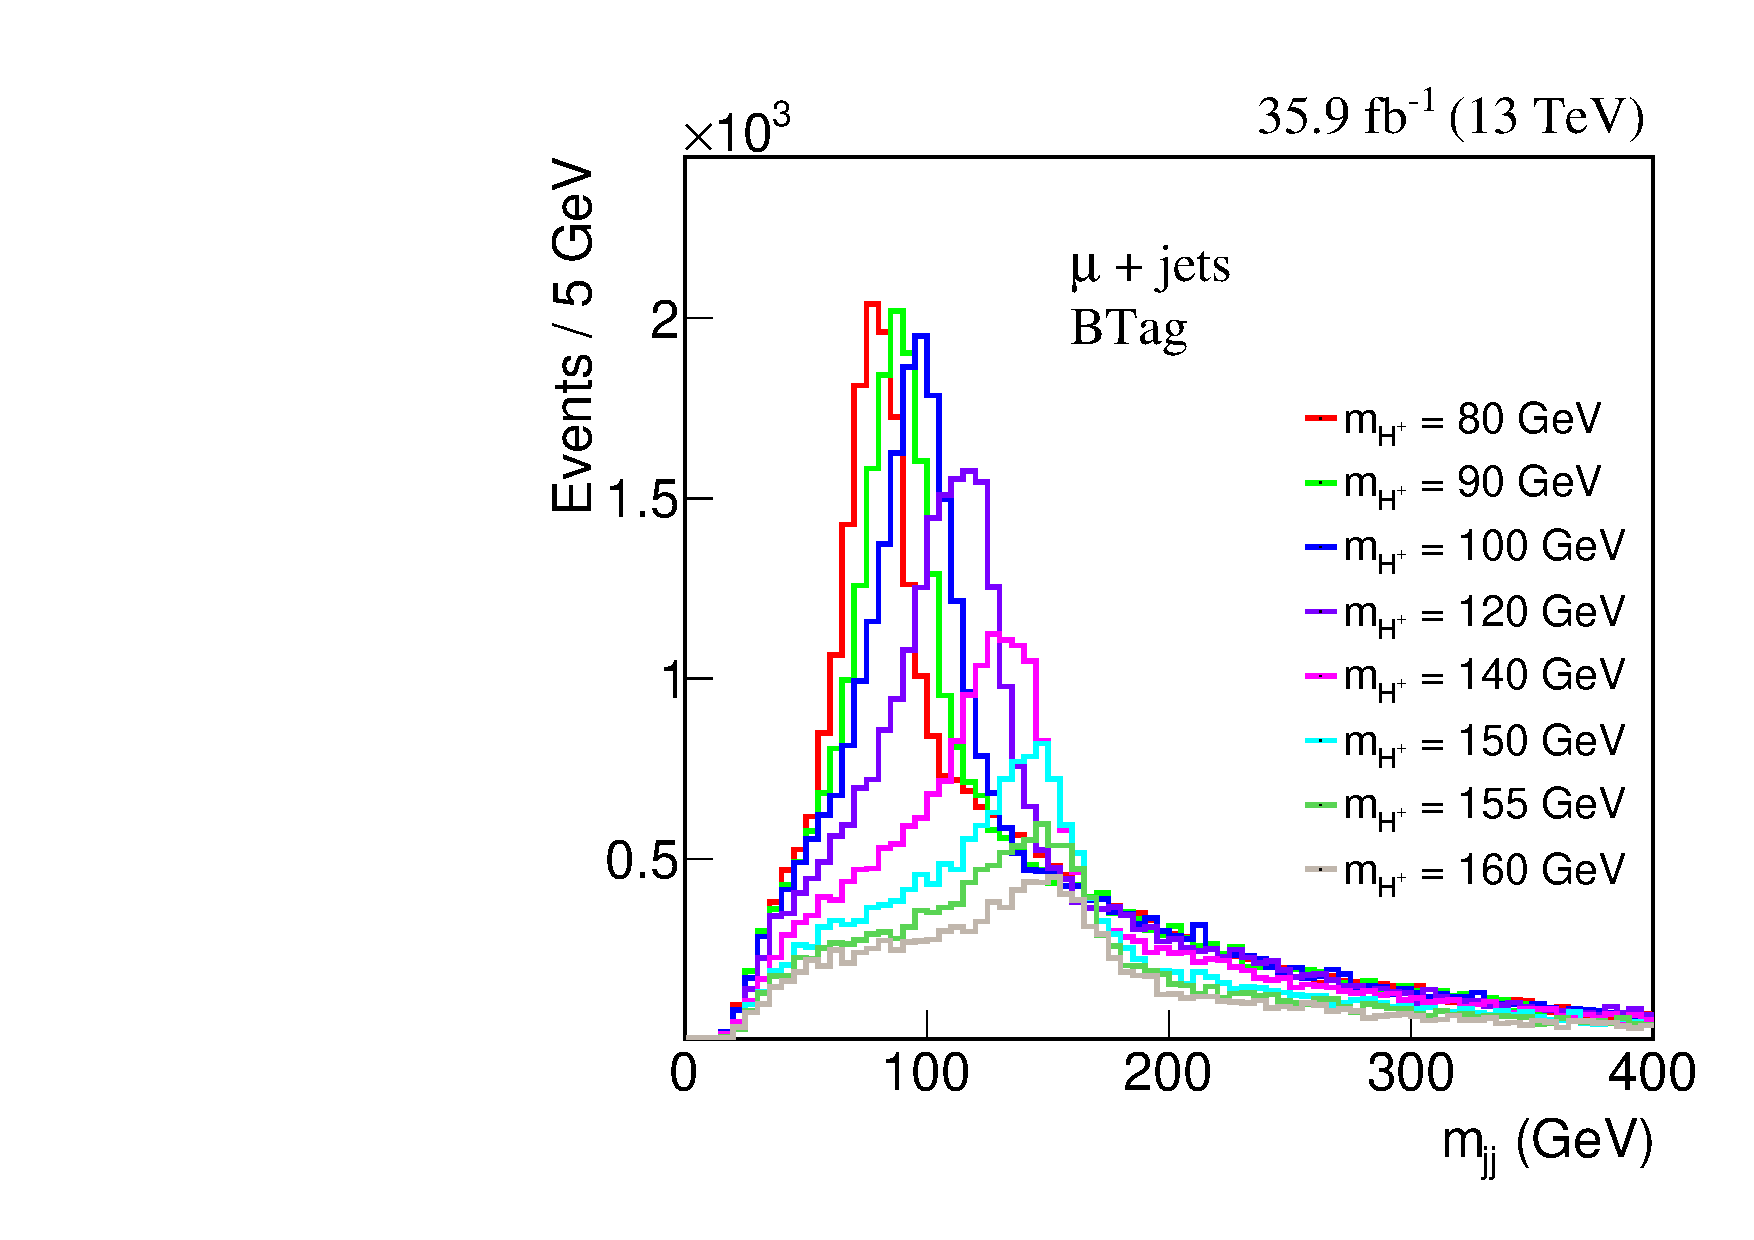
\includegraphics[width=0.45\linewidth]{Image/Muon/MjjShape_mu/sig_BTag_mjj_mu.pdf}}
    \subfigure[With reconstructed jets \label{subfig:mjj_sig_btag_ele}]
    {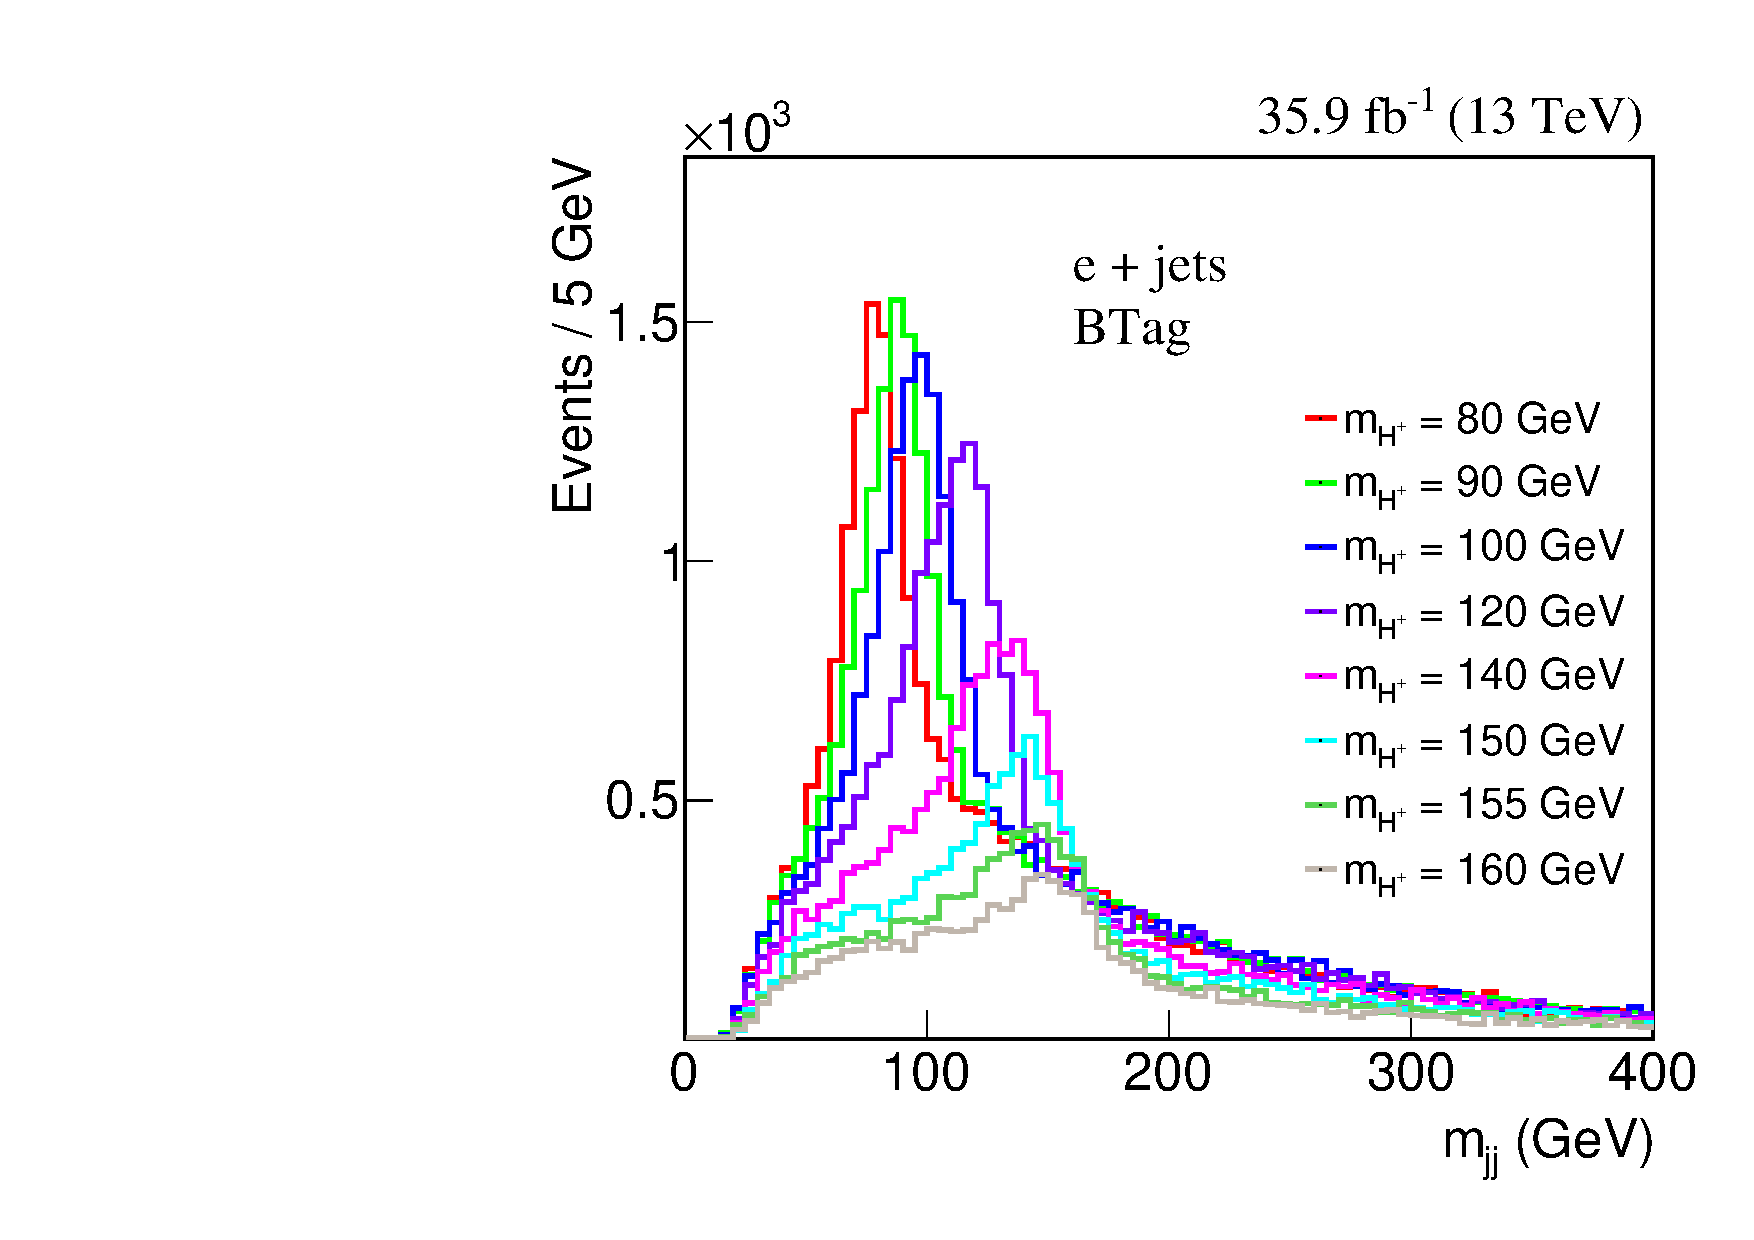
\includegraphics[width=0.45\linewidth]{Image/Electron/MjjShape_ele/sig_BTag_mjj_ele.pdf}}
    \vfil
    \subfigure[With kinematic fitted jets \label{subfig:mjj_sig_kfit_mu}]
    {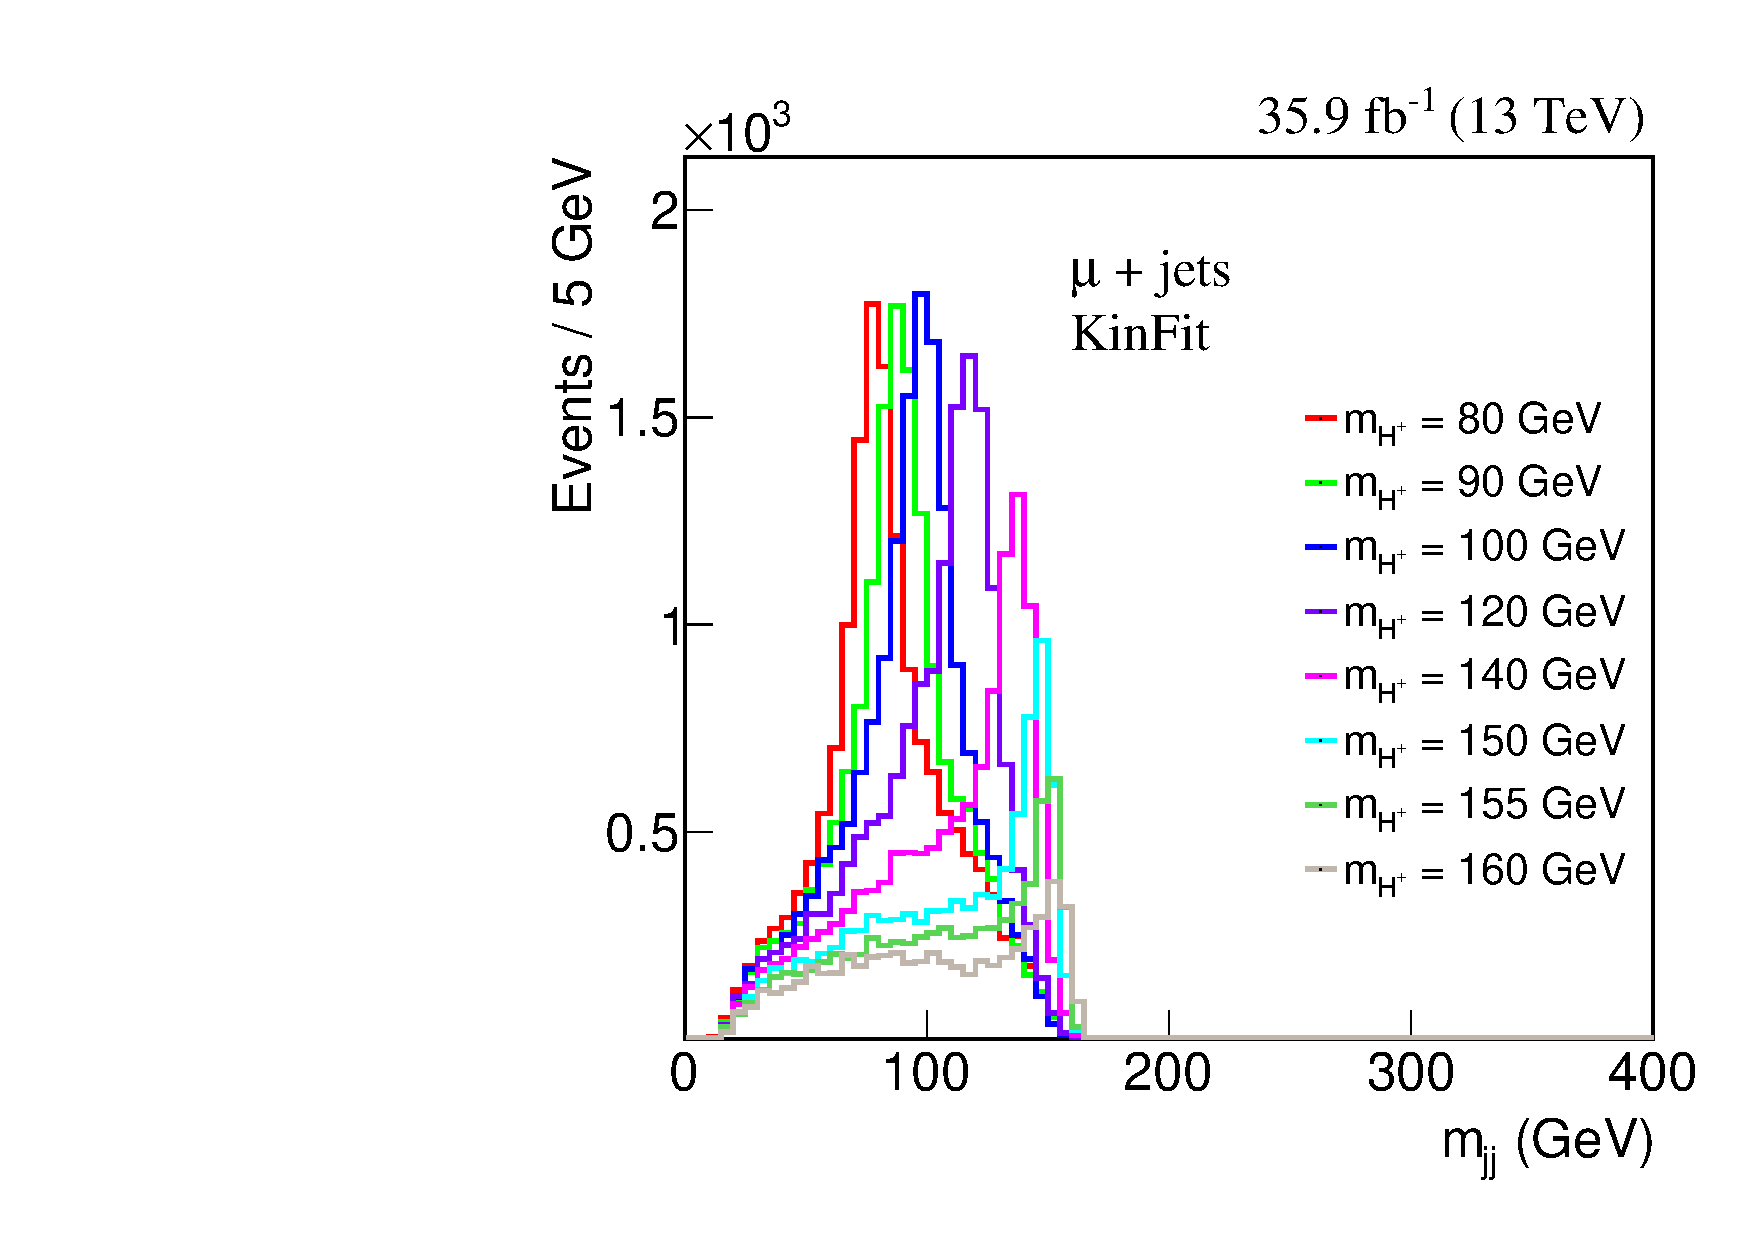
\includegraphics[width=0.45\linewidth]{Image/Muon/MjjShape_mu/sig_KinFit_mjj_kfit_mu.pdf}}
    \subfigure[With kinematic fitted jets \label{subfig:mjj_sig_kfit_ele}]
    {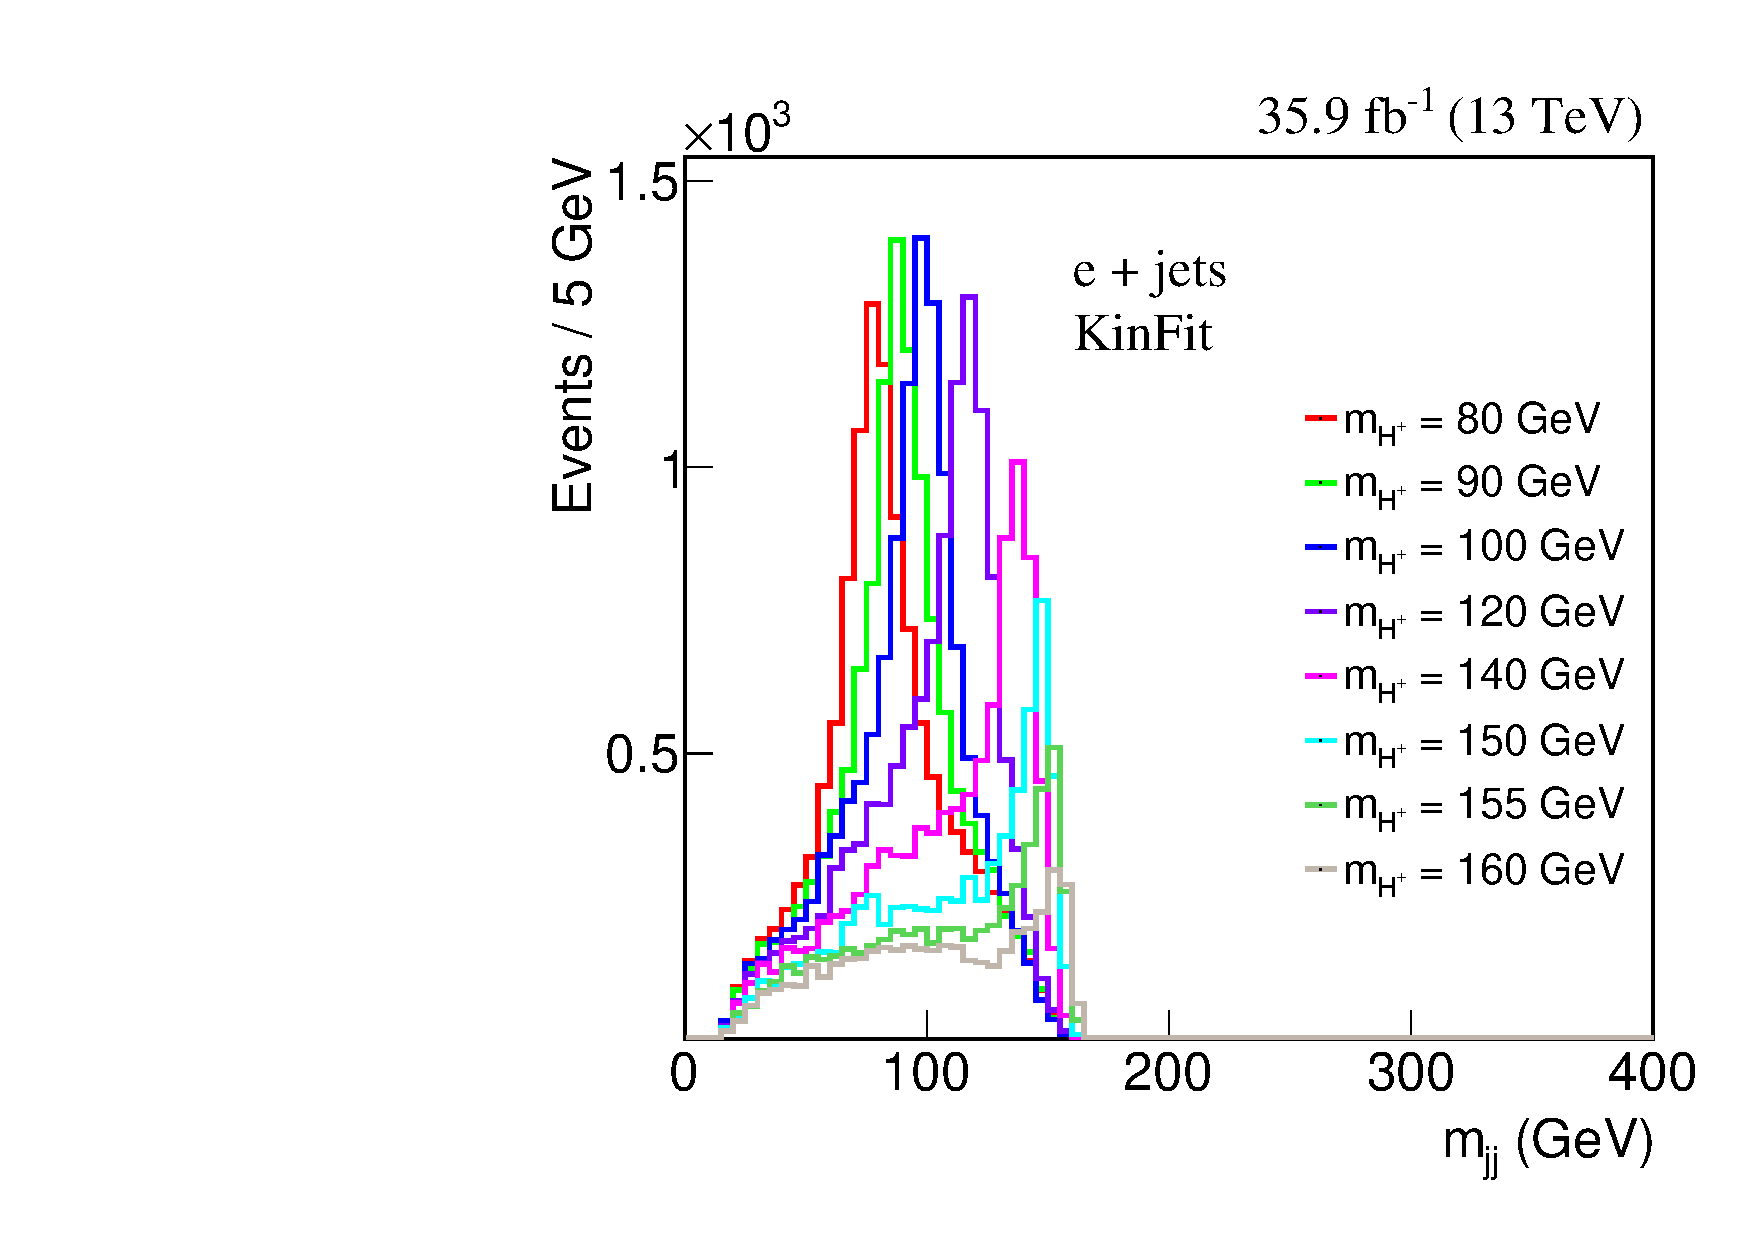
\includegraphics[width=0.45\linewidth]{Image/Electron/MjjShape_ele/sig_KinFit_mjj_kfit_ele.pdf}}
    \caption{$\mjj$ distributions of two non \PQb, highest \pt jets from charged
        Higgs signal samples ($\mHp$ = 80, 90, 100, 120, 140, 150, 155, 
        160 \GeV) for \mujets and \ejets channel. The $\mjj$
        distributions of Figures~\ref{subfig:mjj_sig_btag_mu}, 
        \ref{subfig:mjj_sig_btag_ele} are evaluated using reconstructed jets 
        after \PQb jet selection. Whereas $\mjj$ distributions of 
	Figures~\ref{subfig:mjj_sig_kfit_mu}, \ref{subfig:mjj_sig_kfit_ele} are evaluated 
	using kinematic fitted jets after kinematic fit selection.} 
    \label{fig:mjjBTagKinFit_Sig}
\end{figure}

